\chapter{L'entreprise et la bourse}

\section{Nature et forme des entreprises}

\begin{itemize}
    \item \textblue{SLR} - Société à Responsabilité Limitée
    \item \textblue{SA} - Société Anonyme
    \item \textblue{SC} - Société Coopérative
\end{itemize}

\section{Séparation propriété-gestion}

\begin{itemize}
    \item Dans une SA, la propriété et le contrôle sont distincts
    \item Assemblée générale des actionnaires
    \begin{itemize}
        \item Approuve les comptes annuels et la politique de rémunération des actionnaires
        \item Désigne les administrateurs
        \item Donne d"charge aux administrateurs et réviseurs
    \end{itemize}
    \item Le conseil d'administration
    \begin{itemize}
        \item Désigne un (ou plusieurs) administrateurs délégués à la gestion journalière, généralement le CEO
    \end{itemize}
    \item Chief Financial Officer (CFO)
    \begin{itemize}
        \item Gère les décisions d'investissement, financement et pour la trésorerie
    \end{itemize}
\end{itemize}

\section{Regard critique}

Le management prend des décisions afin de maximiser la valeur de l'entreprise
\begin{itemize}
    \item Sans porter préjudice à l'ensemble des stakeholders
    \item Dans le respect de l'éthique et de l'environnement
    \item Volonté d'impact sur la société et l’environnement (SDG - Sustainable Development Goods)
    \item[$\rightarrow$] Corporate Sustainability Reporting Directive (CSRD)
\end{itemize}

\section{Les marchés boursiers}

\begin{itemize}
    \item \textblue{Marchés primaires} : ex. Lorsque l'entreprise lève des fonds
    \item \textblue{Marchés secondaires} : Une fois les titres émis sur le marché primaire, ils sont négociés sur le marché secondaire
    \item \textblue{Actions} :
    \begin{itemize}
        \item Participation au capital d'une entreprise
        \item Potentiel élevé de rendement, mais avec des fluctuations importantes $\rightarrow$ risque plus élevé
    \end{itemize}
    \item \textblue{Obligations} :
    \begin{itemize}
        \item Prêt à une entité avec engagements de remboursement avec intérêts
        \item Moins risqué que les actions mais dépend de la quantité de crédit de l'émetteur
        \item Payements d'intérêts réguliers (coupons)
    \end{itemize}
    \item \textblue{Cash} : 
    \begin{itemize}
        \item Comptes épargnes, dépôts à vue
        \item Risque très faible mais rendement nul
    \end{itemize}
\end{itemize}

\addtocounter{chapter}{1}
\chapter{Arbitrage et décisions financières}

\section{Décisions financières}

Basées uniquement sur des valeurs actualisées (VA)

\section{Taux d'intérêt et valeur temporelle de l'argent}

Exemple : nous investissons de 100€ à 5\% sur 1 an :
\begin{itemize}
    \item 100€ correspond à la valeur actuelle (VA)
    \item 5\% correspond au taux d'actualisation de taux sans risque (E(R))
    \item la valeur future (VF)  est égale à $100 + 100 * 0.05 = 105$€
\end{itemize}

\begin{itemize}
    \item[$\hookrightarrow$] \textblue{Return} $= 5\% = \frac{105-100}{100} \rightarrow 100 = \frac{105}{1 + 0.05}$
    \item[$\hookrightarrow$] \textblue{$VA$} $= \frac{VF}{1 + E(R)} \leftrightarrow \textblue{VF} = VA * (1 + E(R))$
\end{itemize}

\section{La valeur actuelle et la règle de décision VAN}

\begin{itemize}
    \item \textblue{Valeur Actuelle Nette} (VAN) = valeur actuelle des recettes (cashflow > 0) - valeur actuelle de ses coûts (cashflow < 0)
    \item \textblue{Règle de décision} :
    \begin{itemize}
        \item[\textgreen{V}] si VAN $\geq 0 \rightarrow$ favorable de maximiser la VAN
        \item[\textred{X}] si VAN $< 0$
        \item Si toutes les options d'investissement sont à un an et sans risque $\rightarrow$ taux d'actualisation = 2\%
    \end{itemize}
\end{itemize}

\section{Arbitrage et la loi de prix unique}

\begin{itemize}
    \item \textblue{Arbitrage} :
    \begin{itemize}
        \item Achat-revente de biens équivalents sur des marchés différents pour profiter d'une différence de prix
        \item Possibilité de réaliser un profit sans prendre de risque ni faire d'investissements
    \end{itemize}
    \item \textblue{Marché normal} : marché concurrentiel sans opportunités d'arbitrage
    \item \textblue{Loi du prix unique} : si des opportunités d'investissement se présentent sur différents marchés concurrentiels, elles doivent se négocier au même prix
\end{itemize}

\section{Absence d'arbitrage et valeurs des titres}

Si le prix = $940$€ :
\begin{itemize}
    \item[$\rightarrow$] Achat de l'obligation et emprunt à 1 an de $1000$€ à 5\%
    \item Cash de l'emprunt : $VA = \frac{100}{1.05} = 952.4$€ $\rightarrow$ on reçoit ajd $952.4$€
    \item Cash de l'achat de l'obligation : $-940$€
    \item Solde : $952.4 - 940 = 12.4$€ $\rightarrow$ cash directement en poche
\end{itemize}
Dans 1 an :
\begin{itemize}
    \item Remboursement du prêt : $-1000$€
    \item Récupération de la valeur de l'obligation : $+1000$€
    %\item Total : $0$€
\end{itemize}

\chapter{La valeur temps de l'argent}

\section{L'échéance}

ou diagramme des flux :
\begin{figure}[H]
    \centering
    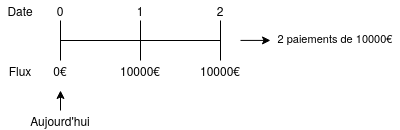
\includegraphics[width=0.57\textwidth,keepaspectratio]{flux}
\end{figure}

\section{Actualisation - Capitalisation}

\begin{itemize}
    \item[$\rightarrow$] Permet de comparer des sommes disponibles à des dates différentes
    \item \textblue{Capitalisation} : présent $\rightarrow$ avenir
    \item \textblue{Actualisation} : présent $\leftarrow$ avenir
    \item Capitalisation - intérêts composés :
    \begin{itemize}
        \item[$\rightarrow$] La VF d'un placement en $0$ pour $t$ périodes au taux d'intérêt composé $i$ est égal à :
        \begin{align*}
            &VF(A@i\%) = A * (1 + i)^t &&&&& (t > 1 \text{ an})
        \end{align*}
    \end{itemize}
    \begin{itemize}
        \item[$\rightarrow$] Si intérêt simple :
        \begin{align*}
            &VF(A@i\%) = A * (1 + i * t) & (t < 1 \text{ an, ex : 3 mois}\rightarrow t = 0.25)
        \end{align*}
    \end{itemize}
    \item Ex : on propose un investissement donnant un cashflow de 121€ dans 2 ans. On attend un return de 10\%. On investit combien ? $VA = \frac{121}{(1 + 0.1)^2} = 100$€
    \item[$\rightarrow$] Valeur actuelle d'un cashflow A : $VA (A@i\%) = \frac{A}{(1 + I)^t}$
\end{itemize}

\section{Valeur actuelle et future d'une séquence de flux}

\begin{align*}
    VF &= A * \left[ \frac{(1 + i)^n - 1}{i}         \right] \\
    VA &= A * \left[ \frac{1 - 1/(1+i)^n}{i} \right]
\end{align*}

Ex : Quel montant $x$ faut-il épargner annuellement au cours des $20$ prochaines années afin de percevoir une rente annuelle de $10000$€ pour les 20 prochaines années qui suivent ? Le taux d'intérêt est de 5\%.
\begin{itemize}
    \item[$\rightarrow$] La valeur future de $x$ à l'année 20 doit être égale à la valeur actuelle de $A$ à l'année $20$ :
\end{itemize}
\begin{align*}
    x * \left( \frac{(1 + 0.05)^{20} - 1}{0.05} \right) &= 10000 * \left( \frac{1 - 1/(1 + 0.05)^{20}}{0.05} \right) \\
    \Leftrightarrow x &= 3.769
\end{align*}

\section{Rentes perpétuelles, annuités et autres cas particuliers}

\begin{itemize}
    \item Valeur actuelle au taux $i$ d'un cashflow constant $A$ :
    \begin{align*}
        VA = \frac{A}{i}
    \end{align*}
    \item Valeur actuelle au taux $i$ d'i, cashflow $A$ de croissance constante $g < i$ :
    \begin{align*}
        VA = \frac{A_1}{i - g} && A_t = A_1 * (1 + g) t - 1
    \end{align*}
\end{itemize}

\section{Valeur actuelle nette d'une séquence de flux}

VAN = valeur actuelle de tous les cashflows d'un projet :
\begin{align*}
    VAN = \sum_{t = 0}^T \frac{CF_t}{(1 + E(R))^t}
\end{align*}

\section{Flux infra-annuels}

\warning Cohérence des unités : les périodes et le taux d'actualisation doivent être exprimés dans les mêmes unités (ex : périodes annuelles et taux annuel ou périodes mensuelles et taux mensuels)

\section{Calculer les montants à payer, le TRI, le nombre de périodes}

\begin{itemize}
    \item \textblue{TAEG} : Taux Annuel Effectif Global
    \item \textblue{TRI} : Taux de Rentabilité Interne
    \begin{itemize}
        \item[$\rightarrow$] Taux d'actualisation des cashflows t.q. $VAN = 0$
        \item[$\rightarrow$] $VAN = 0 = \sum_{t = 0}^T \frac{CF_t}{(1 + TRI)^t}$
        \item Correspond à la rentabilité attendue d'un projet
    \end{itemize}
\end{itemize}

\textblue{Note} : lorsqu'il s'agit d'un financement (CF > 0 suivi de paiements) TRI = coût d’emprunt)

\addtocounter{chapter}{1}
\chapter{La valorisation des obligations}

\textblue{Définition} : titre obligeant l'émetteur à effectuer des paiements déterminés au détenteur de l'obligation.

\section{Caractéristiques des obligations}

\begin{itemize}
    \item \textblue{Émetteur}
    \begin{itemize}
        \item Gouvernement
        \item Corporate : Junior (obligations remboursées après Senior, Risque $\nearrow$ : taux d'intérêt $\nearrow$) vs Senior (remboursés en premier)
    \end{itemize}
    \item \textblue{Fréquence de coupon} : paiements des intérêts aux obligataires
    \item \textblue{Taux de coupon}
    \item \textblue{Valeur nominale} : Généralement remboursée à la maturité
    \item \textblue{Cotation} :
    \begin{itemize}
        \item Un pourcentage de la valeur nominale
        \item Intérêt connu
    \end{itemize}
    \item \textblue{Rating} : de AAA (très safe) à C (pas safe du tout ; prime de risque $\nearrow$ (spread))
    \begin{itemize}
        \item[$\rightarrow$] \textblue{Taux de défaut} : probabilité que l'émetteur de l'obligation ne puisse pas honorer ses paiements d'intérêts ou rembourser le capital à l'échéance
        %\item \textblue{Note} : plus le spread $\nearrow$ plus le taux de défaut $\nearrow$
    \end{itemize}
    \item \textblue{Corporate bonds} : titres de créances émis par des entreprises pour lever des fonds
    \begin{itemize}
        \item Classement : Haute qualité (> BBB) $\rightarrow$ Haute performance (BB <)
    \end{itemize}
    \item Dirty price = clean price + intérêt couru
    \item[$\hookrightarrow$] intérêt couru = coupon annuel $* \frac{\text{\# jours écoulés}}{\text{\# jours entre 2 paiements}}$
\end{itemize}

\section{Prix et yields}

\begin{itemize}
    \item \textblue{Prix des obligations} (PV) : valeur actuelle des flux de trésorerie futures
    \begin{align*}
        PV &= \sum_{t = 1}^T \frac{CF_t}{(1+E[R])^t}\\
           &= \sum_{t=1}^T \frac{C}{(1+E[R])^t} + \frac{R}{(1 + E[R])^T}\\
           &= C * \left[ \frac{1 - 1/(1+E[R])^T}{E[R]} \right] + \frac{R}{(1 + E[R])^T}
    \end{align*}
    Où :
    \begin{itemize}
        \item $C$ = paiement périodique du coupon
        \item $R$ = remboursement final (souvent égal à la valeur nominale)
        \item $E[R]$ = rendement
    \end{itemize}
    \item Si le taux d'intérêt du marché est supérieur (inférieur) au taux du coupon, les obligations se vendent à un prix inférieur (supérieur) à leur valeur nominale
    \item \textblue{Current yield} = coupon annualisé divisé par le prix
    \item \textblue{Yield to Maturity} (YTM) = taux d'actualisation (return attendu) pour lequel la valeur actuelle des flux futurs est égal au prix (dirty price) actuel
    \item \textblue{Premium bond} (prix > valeur nominale) : Current Yield > YTM
    \item \textblue{Discount bond} (prix < valeur nominale) : Current Yield < YTM
    \item \textblue{Rate of return} : revenu total (coupon + variations de prix) par période et euro investi
    \item[$\hookrightarrow$] $R = \frac{P_1 - P_0}{P_0} + \frac{C}{P_0}$
    \begin{itemize}
        \item[$=$] YTM si intérêt stable et l'obligation est conservée jusqu'à échéance
    \end{itemize}
\end{itemize}

\subsection{Current Yield VS YTM}

\begin{itemize}
    \item \textblue{Current yield} : 1er indicateur du rendement d'une obligation mais pas précis car il ne prend pas en compte la génération de gais ou pertes
    \item \textblue{YTM} mesure plus précise, prend en compte les flux de trésorerie et l'écart entre le prix d'achat actuel et la valeur de remboursement de l'obligation à échéance
\end{itemize}

\section{Risque de taux}

\begin{itemize}
    \item Les obligations à long-terme sont plus sensibles aux variations des taux d'intérêt que celles à court-terme
    \begin{itemize}
        \item[$\rightarrow$] si le taux d'intérêt $\nearrow$, plus l'obligation est longue, plus la perte d'opportunité grandie
    \end{itemize}
    \item \textblue{Volatilité des obligations} : diminue (augmente) si le rendement augmente (diminue)
    \item \textblue{Risque de taux d'intérêt} : le détenteur de l'obligation décide de la vendre avant son échéance (souvent car le taux d'intérêt augmente)
    \item \textblue{Duration} (D) : évalue la sensibilité du prix d'une obligation à une variation des taux d'intérêt :
    \begin{align*}
        D &= \sum_{t=1}^T w_t * t \text{, avec } w_t = \frac{CF_t}{(1+YTM)^t} / \sum_{k=1}^T \frac{CF_k}{(1 + YTM)^k}
    \end{align*}
\end{itemize}

\section{Arbitrage: Taux variable vs Taux fixe à long terme}

\begin{itemize}
    \item Taux variable (taux de référence + spread)
    \begin{itemize}
        \item Financement à un taux plus faible
        \item Risque sur la charge d'intérêt
        \item La prime de risque (spread) est fixe
    \end{itemize}
    \item Taux fixe
    \begin{itemize}
        \item Taux plus élevé
        \item Pas de risque sur la charge d'intérêt
    \end{itemize}
\end{itemize}

\section{Prime de risque (spread)}

\begin{itemize}
    \item[$=$] différence de rendement entre une obligation du Trésor équivalente et une obligation d'entreprise
    \item Fonction de :
    \begin{itemize}
        \item Probabilité de défaut ($\lambda$)
        \item Taux de recouvrement ($R$)
        \item Prix du risque sur le marché ($r$)
    \end{itemize}
    \item[$\rightarrow$] Spread = $\lambda (r - R)$, où $\lambda$ est la probabilité de défaut, et $R$ le taux de recouvrement
\end{itemize}

\chapter{Règles de décision et d'investissement}

\section{La valeur actuelle nette}

\begin{itemize}
    \item[$=$] valeur actuelle de tous les cashflows
    \begin{align*}
        VAN = \sum_{t=0}^T \frac{CF_t}{(1 + E[R])^t}
    \end{align*}
    \item[$\hookrightarrow$] si $VAN > 0$ :
    \begin{itemize}
        \item VA des investissements < VA des cashflows générés par l'investissement
        \item valeur de l'entreprise $\nearrow$
        \item l'entreprise va réussir à récupérer le capital investi, rémunérer les bonds immobilisés selon les exigences des investisseurs, dégager du surplus pour les actionnaires dont la VA est égale à la VAN du projet
    \end{itemize}
    \item taux d'actualisation = coût d'opportunité du capital, c-à-d la rentabilité à laquelle les investisseurs renoncent pour entreprendre le projet
    \item risque intégré via le taux de rentabilité attendu
\end{itemize}

\section{Taux de rentabilité interne}

\begin{itemize}
    \item \textblue{Hypothèse de réinvestissement} : Pour que la rentabilité d’un investissement soit égale au TRI, il est indispensable que l’investissement soit maintenu jusqu’à la date de fin et que tous les cashflows intermédiaires soient réinvestis dans des projets de rentabilité égale au TRI
    \item \textblue{Critère de décision} : tout projet dont TRI > coût d'opportunité du capital devrait être accepté
    \item Critère de VAN préférable car en ligne avec l'objectif de maximisation de la valeur et ne fait pas l'hypothèse de réinvestissement (contrairement au TRI)
\end{itemize}

\section{Délai de récupération (payback)}

\begin{itemize}
    \item[$=$] temps nécessaire pour que les cashflows remboursent l'investissement initial
    \begin{align*}
        \sum_{t=1}^{payback} CF_t - I_0 \geq 0
    \end{align*}
    \warning Ne tient pas compte de tous les cashflows réalisés après le payback
    \item[$\rightarrow$] \textblue{Délai de récupération actualisé (Discount payback)} = temps nécessaire pour que la VAN des cashflows cumulés actualisés devienne > 0
    \begin{align*}
        \sum_{t=1}^{payback} \frac{CF_t}{(1 + E[R])^t} - I_0 \geq 0
    \end{align*}
\end{itemize}

\section{L'indice de probabilité}

\begin{itemize}
    \item Mesure la VAN en \% des capitaux investis
    \item Mesure l'efficacité de l'utilisation des ressources
    \begin{align*}
        IP = \frac{VAN}{\sum_{t=0}^T \frac{I_t}{(1+E[R])^t}}
    \end{align*}
\end{itemize}

\chapter{Éléments de la décision d'investissement}

\section{Résultats attendus}

\begin{itemize}
    \item \textblue{Résultats d'exploitation}
    \begin{center}
    \begin{tabular}{|c|l|l|}
    \hline 
    \textgreen{+} & Ventes &  \\ 
    \hline 
    \textred{-} & Coût des unités vendues &  \\ 
    \hline 
    $\hookrightarrow$ & = & \textblue{Gross Profit} \\ 
    \hline 
    \textred{-} & Frais de vente, marketing, administratif & \\ 
    \hline 
    \textred{-} & Frais de R\&D &  \\ 
    \hline 
    \textred{-} & Amortissement &  \\ 
    \hline 
    $\hookrightarrow$ & = & \textblue{Ernings Before Interest and Taxes (EBIT)} \\ 
    \hline 
    \textred{-} & Impôts &  \\ 
    \hline 
    = & \textblue{Résultat net d'exploitation} &  \\ 
    \hline 
    \end{tabular}
    \end{center}
    \item \textblue{Résultats incrémentaux} : comparaison des composantes avec et sans investissement
    \item \textblue{Sunk cost} : cashflows engagés et non récupérables
    \item \textblue{Règle} : si la décision d'investir n'a aucun impact sur un cashflow, alors ce cashflow n'est pas pris en compte dans la décision d'investir
\end{itemize}

\section{Free cashflow et calcul de la VAN}

\begin{itemize}
    \item \textblue{Résultats d'exploitation}
    \begin{center}
    \begin{tabular}{|c|l|}
    \hline 
    \textgreen{+} & Amortissement \\
    \hline 
    \textred{-} & CAPEX \\
    \hline
    \textred{-} & Augmentation BFR \\
    \hline 
    \textgreen{+}/\textred{-} & Cashflows de fin \\
    \hline
    = & \textblue{Free cashflows} \\ 
    \hline 
    \end{tabular}
    \end{center}
    \begin{itemize}
        \item[$\hookrightarrow$] permet d'analyser un projet d'investissement
    \end{itemize}
    \item VAN = $\sum_{t=0}^T \frac{\text{Flux de trésorerie disponible}}{(1+\text{opportunité du capital})^t}$
\end{itemize}

\section{Choix entre des projets}

\begin{itemize}
    \item[$\rightarrow$] Choix de la VAN la + élevé
    \item[\warning] Cas particuliers : projet de remplacement de choix entre différents équipements
    \begin{itemize}
        \item[$\hookrightarrow$] calcul du coût annuel équivalent (CAE)
        \begin{align*}
            VAN = \sum_{t=0}^T \frac{FCF_t}{(1 + E[R])^t} = CAE * \frac{1 - \left(\frac{1}{1 + E[R]} \right)^T}{E[R]}
        \end{align*}
        \item Si frais sur 1 an max : VAN = CAE
    \end{itemize}
\end{itemize}

\chapter{Valorisation des actions}

\begin{itemize}
    \item \textblue{Action} :
    \begin{itemize}
        \item Droit de propriété
        \item Droit aux dividendes
        \item Droit de vote / gestion
        \item[$\rightarrow$] Pour financer des investissements, les entreprises lèvent des capitaux par émissions d'actions
    \end{itemize}
    \item \textblue{Earning Per Share (EPS)} : résultat par action
    \item \textblue{Price Earning Ratio (PER ou P/E)} : utilisé pour évaluer la valorisation d'une entreprise
    \begin{itemize}
        \item[$=$] $\frac{\text{Prix de l'action}}{\text{Résultat par action (EPS)}}$
        \item[$\rightarrow$] Si élevé : peut indiquer que les investisseurs s'attendent à une forte croissance future des bénéfices de l'entreprise. Cependant, peut-être que l'action est surévaluée
        \item[$\rightarrow$] Si faible : action sous-évalué ou entreprise avec des difficultés financières
    \end{itemize}
    \item \textblue{Rendement de l'action / dividend yield}
    \begin{itemize}
        \item[$=$] $\frac{\text{Dividende annuelle par action}}{\text{Prix de l'action}}$
        \item[$\rightarrow$] Si élevé : l'entreprise reverse une par importante de ses bénéfices sous forme de dividendes (attractif pour revenus réguliers) mais peut aussi indiquer un prix d'action bas et des problèmes financiers potentiels
        \item[$\rightarrow$] Si faible : l'entreprise réinvestit une grande partie de ses bénéfices dans la croissance future (attractif car croissance LT)
    \end{itemize}
    \item \textblue{Valeur comptable} (état financier) : application de règles pour enregistrer la valeur des actifs et leur financement
    \item \textblue{Valeur de liquidation} (vente rapide) : montant espéré de la vente des actifs après remboursement de toutes les dettes
    \item \textblue{Valeur de marché} (offre / demande) : valeur économique qui prend en compte :
    \begin{itemize}
        \item les opportunités d'investissement futur
        \item les actifs intangibles t.q. l’organisation, la marque, ...
        \item la capacité des actifs à générer plus de valeur en étant dans l'entreprise (extra earning power)
    \end{itemize}
\end{itemize}

\section{Dividend Discount Model}

\begin{itemize}
    \item \textblue{Prix de l'action} $=$ $P_0 = \frac{D_1 + P_1}{1 + E[R]}$, où :
    \begin{itemize}
        \item $D_1$ = dividende attendue
        \item $P_1$ = prix de vente de l'action
        \item $E[R]$ = rentabilité de l'actionnaire
    \end{itemize}
    \item[$\rightarrow$] la rentabilité attendue inclut un taux de dividende (dividend yield) et une plus-value (capital gain) :
    \begin{itemize}
        \item $E[R] = \frac{D_1}{P_0} + \frac{P_1 - P_0}{P_0}$, où :
        \begin{itemize}
            \item $\frac{D_1}{P_0}$ = dividend yield
            \item $\frac{P_1 - P_0}{P_0}$ = capital gain
        \end{itemize}
    \end{itemize}
    \item Si multi-périodique $P_0 = \sum_{t=1}^N \frac{D_t}{(1 + E[R])^t} + \frac{P_N}{(1 + E[R])^N}$
    \item \textblue{Dividende constant} :
    \begin{align*}
       P_0 = \sum_{t=0}^{\infty} \frac{D}{(1 + E[R])^t} &\xrightarrow{\infty} P_0 = \frac{D}{E[R]} \\
         &\hookrightarrow P_0 = \frac{EPS * (1-b)}{E[R]} = EPS * \frac{1-b}{E[R]}
    \end{align*}
    $\rightarrow$ Prix de l'action = multiple des résultats
    \item \textblue{Croissance constante} : on vérifie que la croissance $g$ du dividende est $g = b * ROE$ (ROE = $\frac{\text{Bénéfices net}}{\text{Capitaux propres}}$)
    \item Dès lors :
    \begin{align*}
        D_t &= D_{t-1} * (1 + g) &&&&&&&&&&\\
        D_t &= D_1 * (1+g)^{t-1} &&&&&&&&&&
    \end{align*}
    \item Le DDM devient :
    \begin{align*}
        P_0 &= \sum^{\infty}_{t=1} \frac{D_1 * (1+g)^{t-1}}{(1+E[R])^t} = \frac{D_1}{E[R] - g} &&&&&&&&
    \end{align*}
    \item[$\hookrightarrow$] aussi appelé le modèle de Gordon et Shapiro
    \begin{align*}
        P_0 &= \frac{D_1}{E[R] - g} & E[R] = \frac{D_1}{P_0} + g &&&&&&&&
    \end{align*}
\end{itemize}
